\section{Stato dell'Arte}

\subsection{Modelli Compartimentali}
In epidemiologia i modelli compartimentali sono una tecnica di modellezione 
generica che si predispone molto bene allo studio complessivo del comportamento
di una malattia infettiva \cite{wiki:Compartmental_models_in_epidemiology}. 
Questa tecnica di modellazione si applica anche ad altre branche della 
scienza, come ad esempio la finanza.

Questa tecnica di modellazione matematica basa il proprio funzionamento 
sull'assunzione che, data una popolazione di individui, questi vengano 
etichettati in maniera differente, in base allo stato di progressione 
della malattia che hanno, o non hanno, contratto. Così facendo si vanno a 
definire dei compartimenti ben separati che possono interagire tra loro, ma 
che rimangono comunque chiaramente distinti l'uni dagli altri.

Il modello che tutt'ora viene usato come riferimento e come base per 
lo studio e modellazione è il così detto modello SIR: Susceptible, Infectious, Recovered.

\begin{figure}
    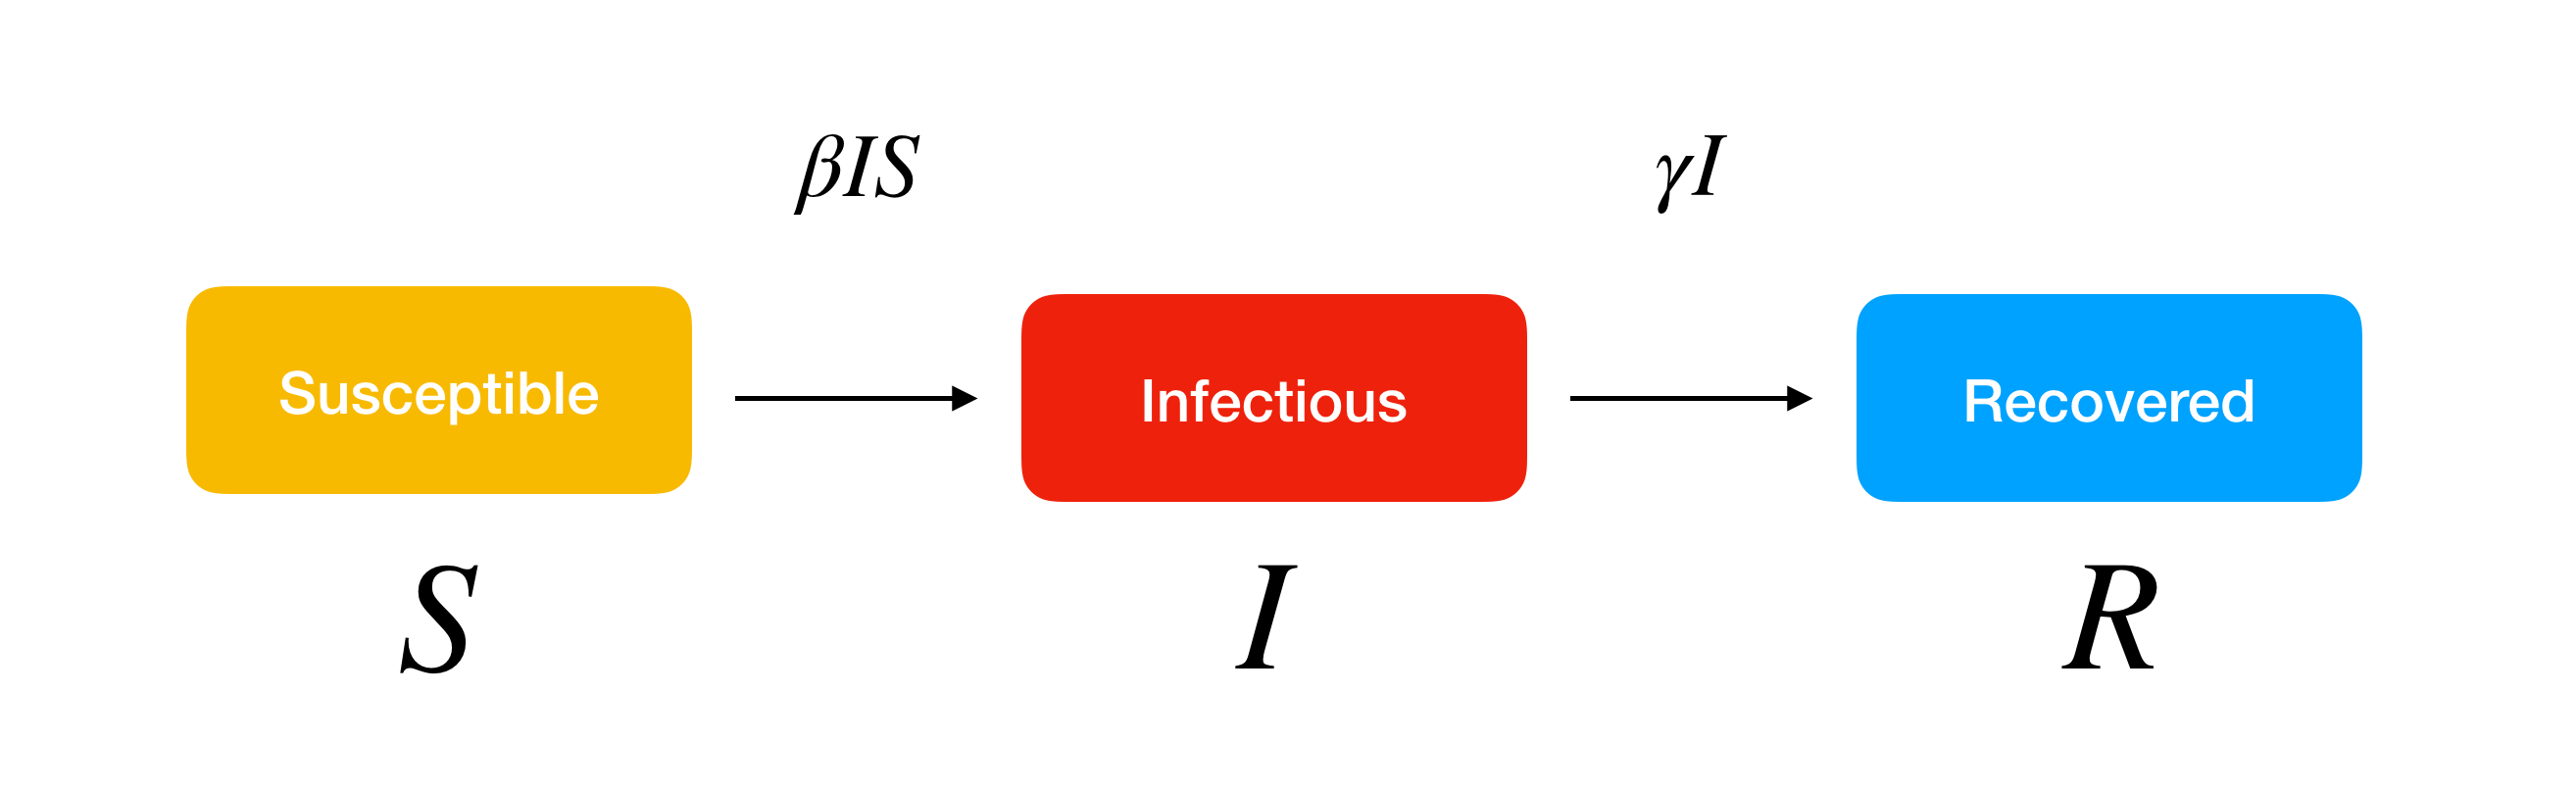
\includegraphics[width=\linewidth]{img/sir.png}
    \caption{Struttura modello SIR} 
    \label{fig:SIR_Structure}
\end{figure}

Questo modello è stato ideato all'inizio del 20esimo secolo, 
più precisamente nel 1917, da Kermack e McKendrick. Come introdotto questo modello
si basa sull'assunzione che all'interno di una popolazione durante 
il decorso di una malattia vi possano esistere solamente tre stadi in cui 
un individuo può essere inserito: 

\begin{itemize}
    \item Susceptible: Questo stadio rappresenta lo stato iniziale per la maggior parte
    degli individui all'interno di una popolazione. Rappresenta il numero di 
    persone che possono contrarre la malattia.
    \item Infectious: Questo stadio rappresenta tutti quegli individui che dallo 
    stato di Susceptible, dopo essere venuti in contatto con un individui infetto, 
    diventano a loro volta individui infetti.
    \item Recovered: Questo stadio rappresenta una duplice categoria, quella degli
    individui che alla fine del docorso della malattia sopravvivono ad essa, e 
    quelli che invece muoiono a causa di questa. Generalemente questo stato viene
    anche definito come Removed.
\end{itemize}

\begin{figure}
    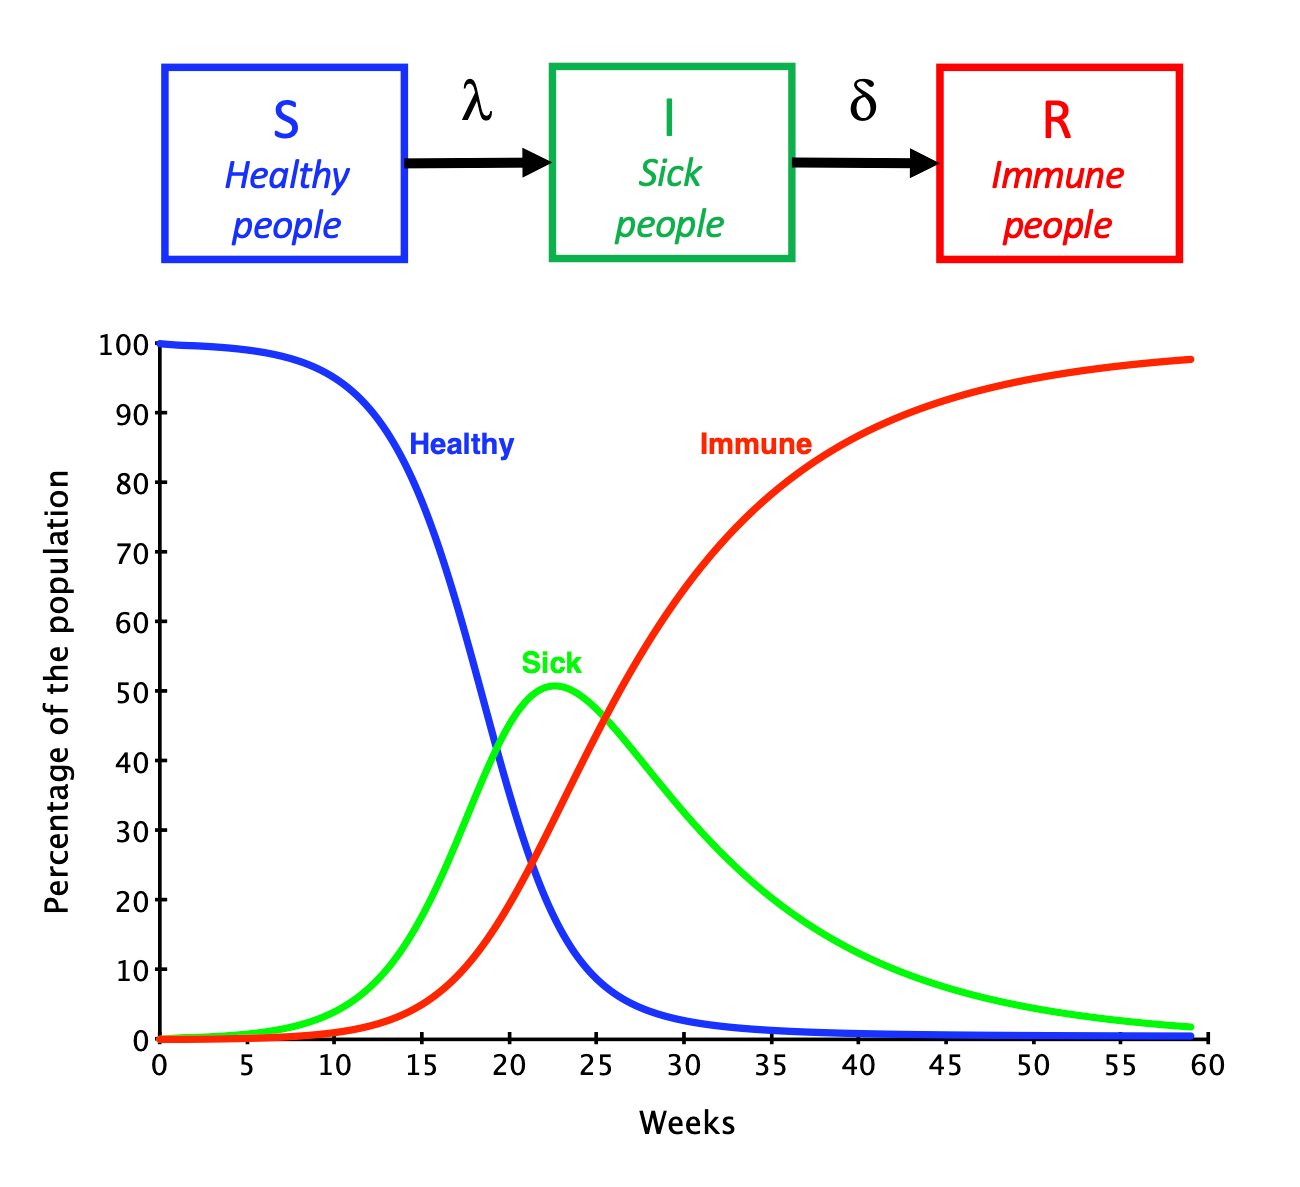
\includegraphics[width=\linewidth]{img/SIR-model.png}
    \caption{Visualizzazione grafico modello SIR} 
    \label{fig:SIR_model_graphic}
\end{figure}

Questo semplice modello funziona grazie all'utilizzo di un sistema di Equazioni
Ordinarie Differenziali (ODE) \cite{Brauer2008}. Una volta definiti i vari parametri inizialo 
utili per la simulazione del decorso di una malattia, è pressocchè immediato trovare
il risultato al tempo T del sistema. Questo modello può essere calcolato tenendo 
in considerazione un andamento più caotico del sistema, utilizzando invece che 
un sistema di ODE, un sistema di SDE \cite{Allen2008} ovvero di Equazioni Differenziali Stocastiche.

\begin{figure}
    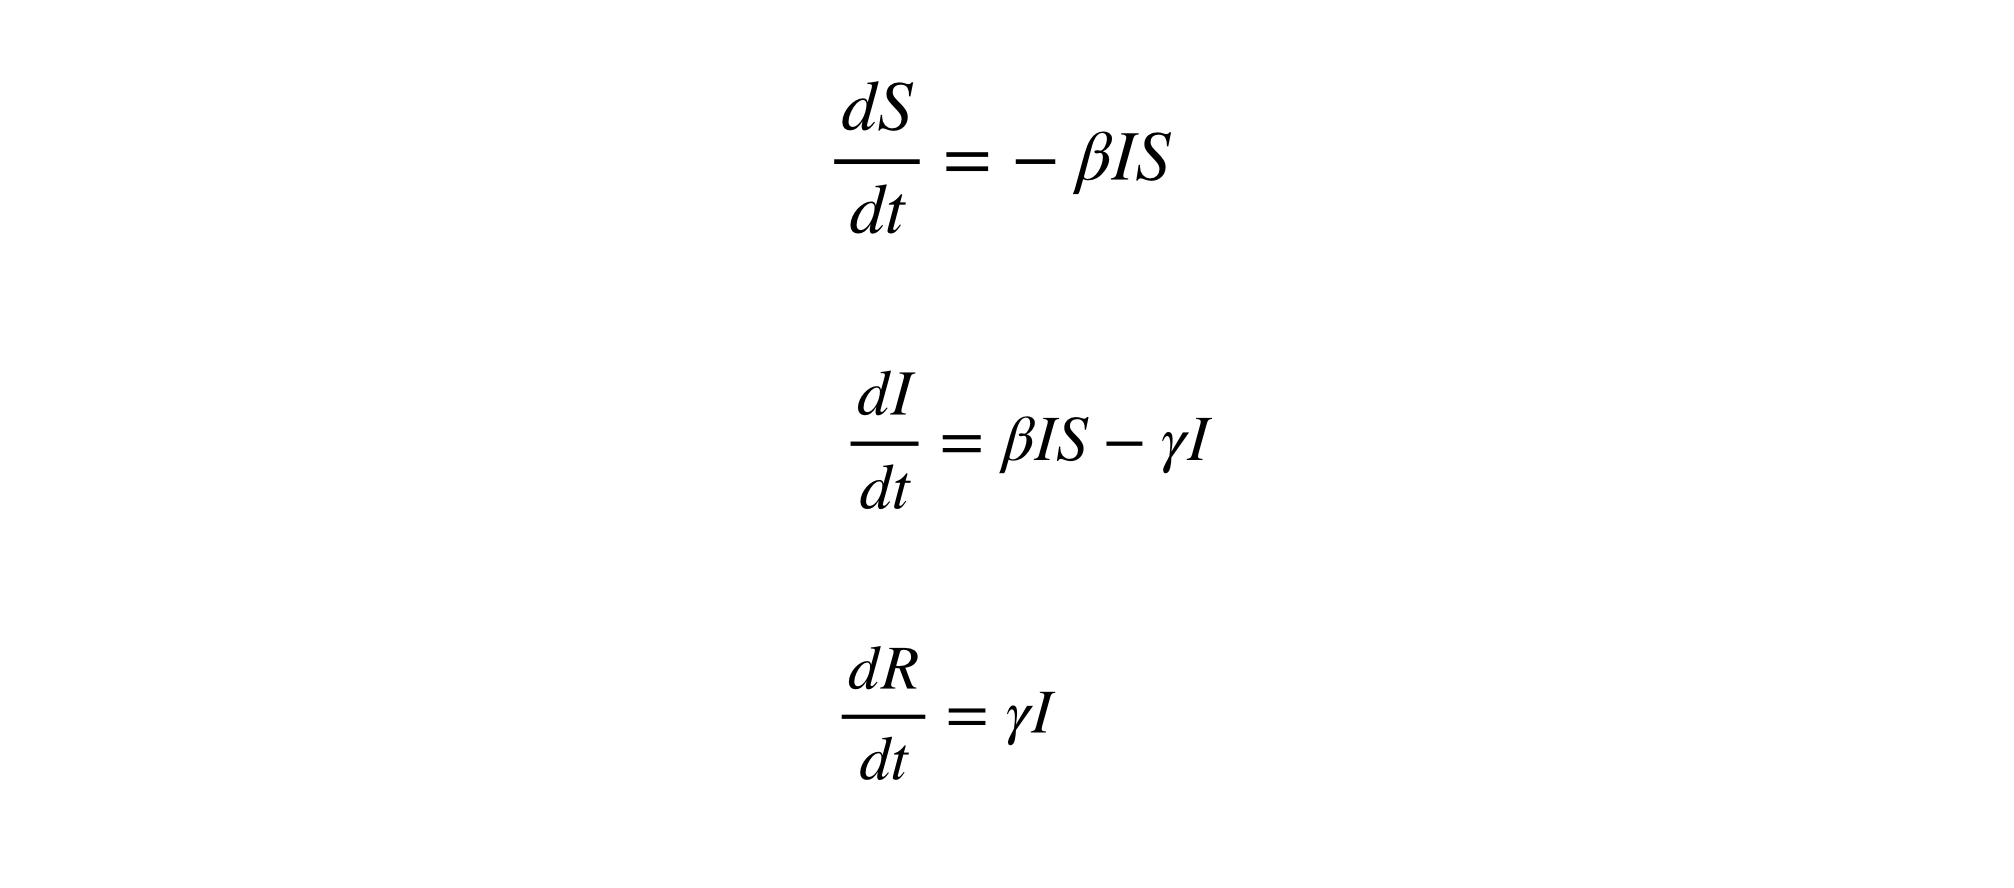
\includegraphics[width=\linewidth]{img/ode.png}
    \caption{Equazioni Ordinarie Differenziali modello SIR} 
    \label{fig:ODE_SIR}
\end{figure}

Con il tempo questo sistema è stato espanso per tenere in considerazione comportamenti
differenti sia della popolazione che delle malattie, andando a definire una moltitudine
di modelli utili a differenti scopi. In epidemiologia tuttavia il modello di
riferimento maggiormente utilizzato è il modello SEIR (Susceptible, Exposed, Infectious, Recovered)
con le sue varianti proprie di ogni approccio \cite{Mwalili2020} \cite{ijerph17103535} \cite{Bjornstad2020}. 
Il motivo per cui viene utilizzato il modello SEIR come base è perchè permette di 
modellare una caratteristica intrinseca di una malattia infettiva, ovvero 
il periodo di latenza che un individuo appena infettato ha prima di diventare 
infettivo a sua volta e mostrare i sintomi di infezione. 

\begin{figure}
    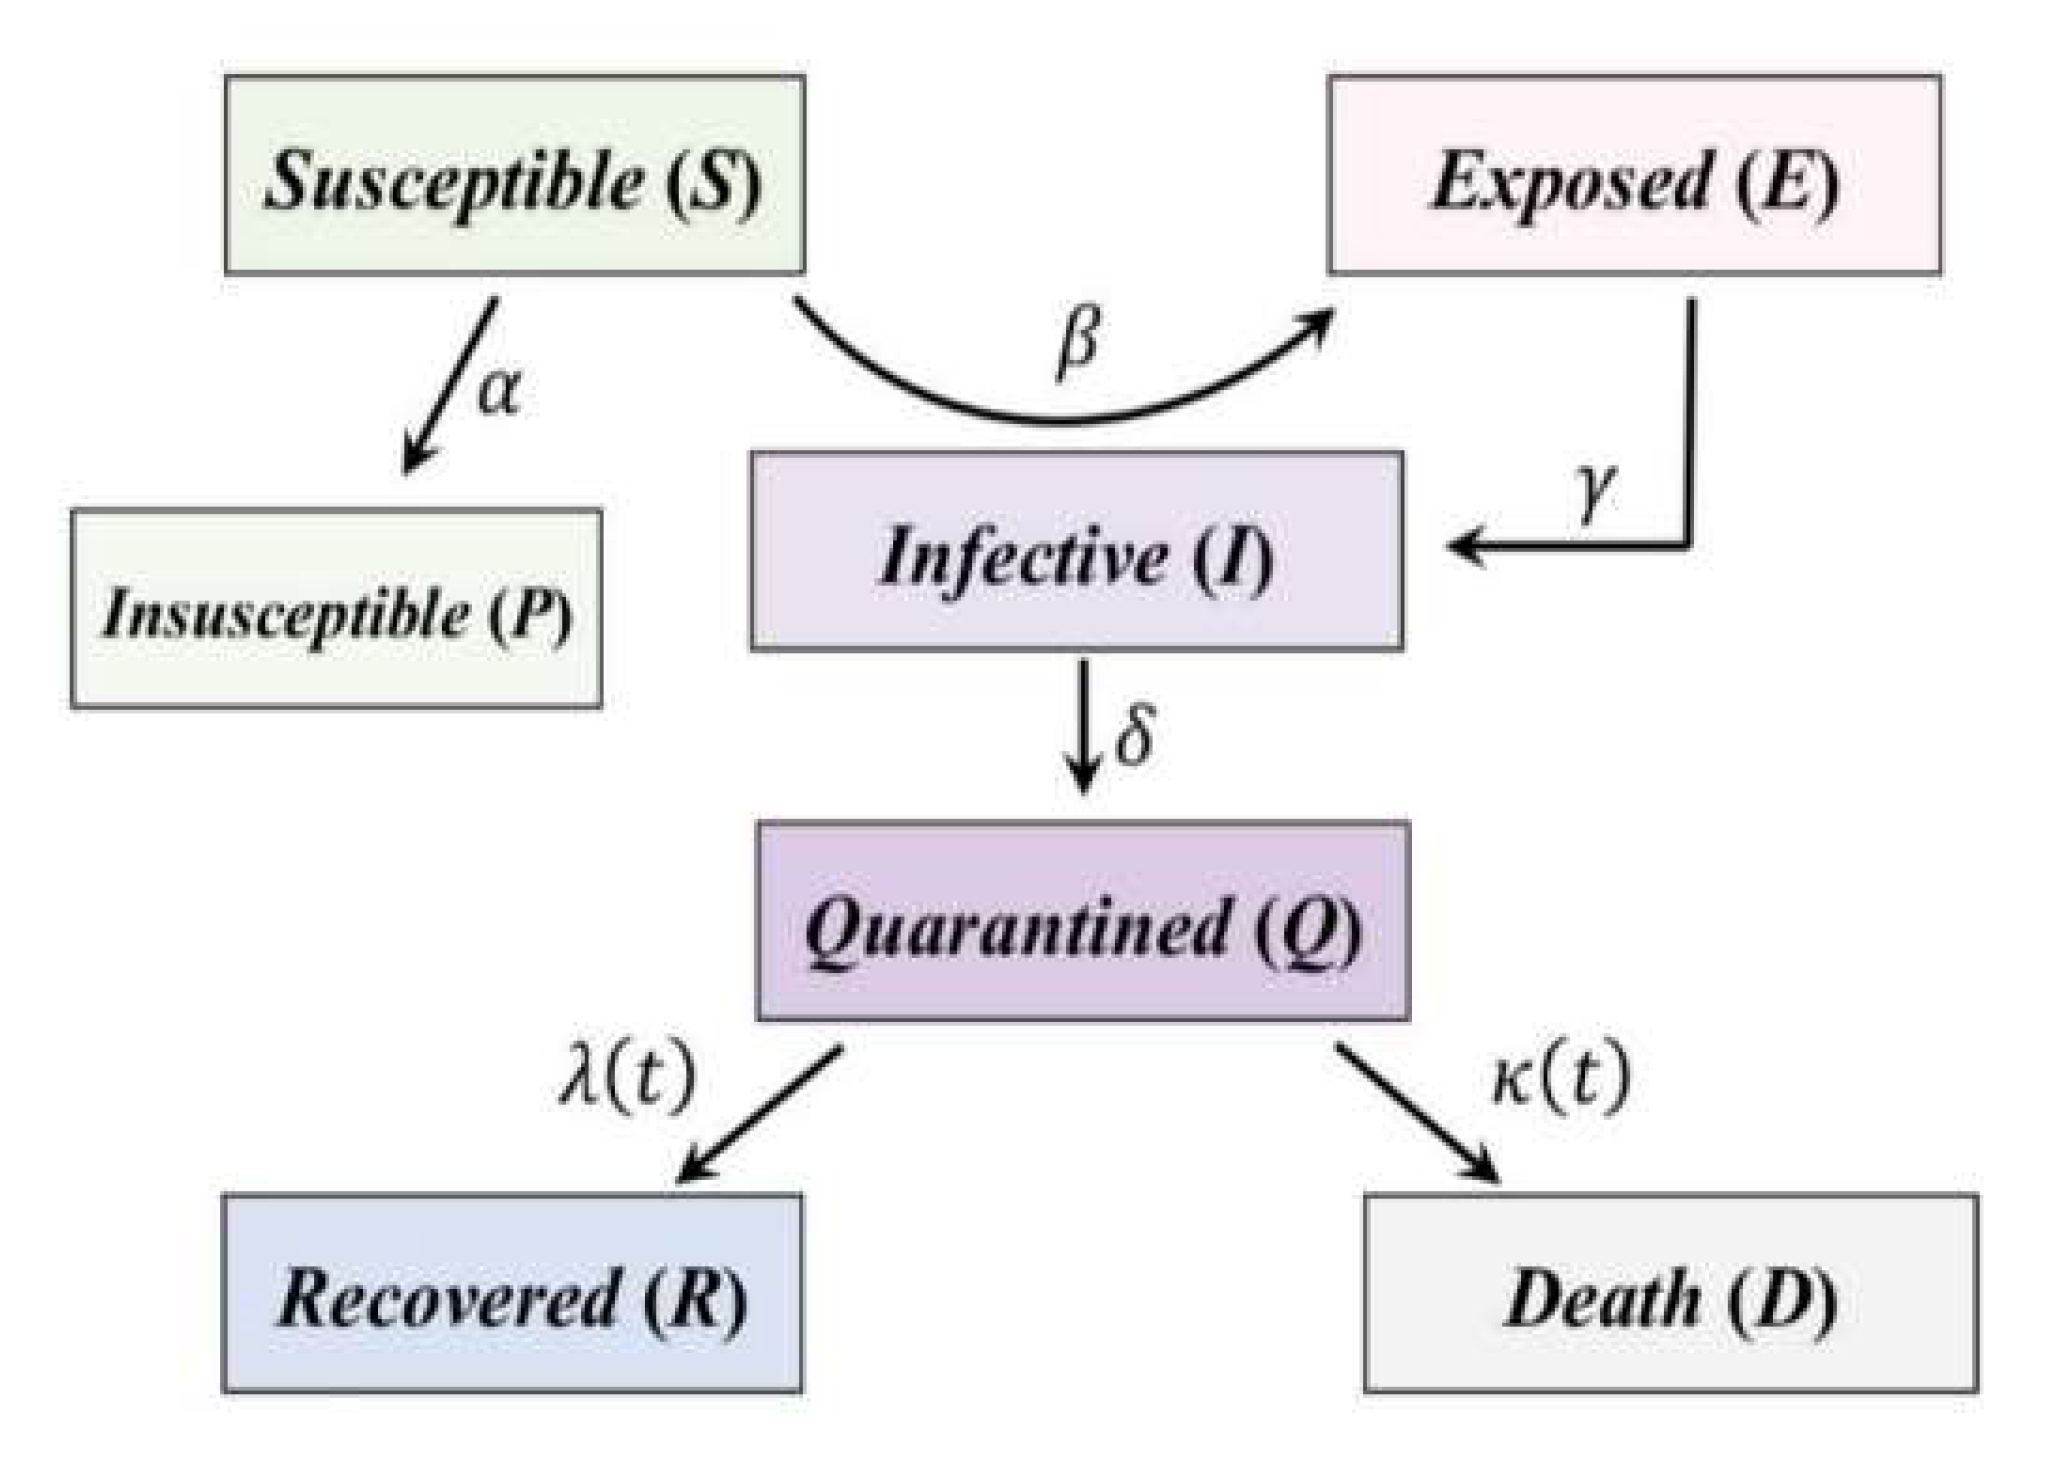
\includegraphics[width=\linewidth]{img/ijerph-17-03535-g001.png}
    \caption{Esempio di modello SEIR preso dall'articolo \cite{ijerph17103535}}
    \label{fig:SEIR_model}
\end{figure}

Una delle modifiche più utilizzate a questo modello è quella di avere un sistema 
ciclico, ovvero in cui gli individui che entrano nello stato R non diventano immuni 
alla malattia a tempo indefinito, ma perdono questa loro caratteristica di immunità
dopo un periodo di tempo. Questo permette di modellare con più accuratezza le malattie
infettive stagionali come ad esempio la comune influenza o il raffreddore, oppure 
mostrare l'andamento ad ondate di altre malattie che hanno la caratteristica di 
mutare molto velocemente, come è stato per il COVID-19 e le sue innumerevoli varianti.

\begin{figure}
    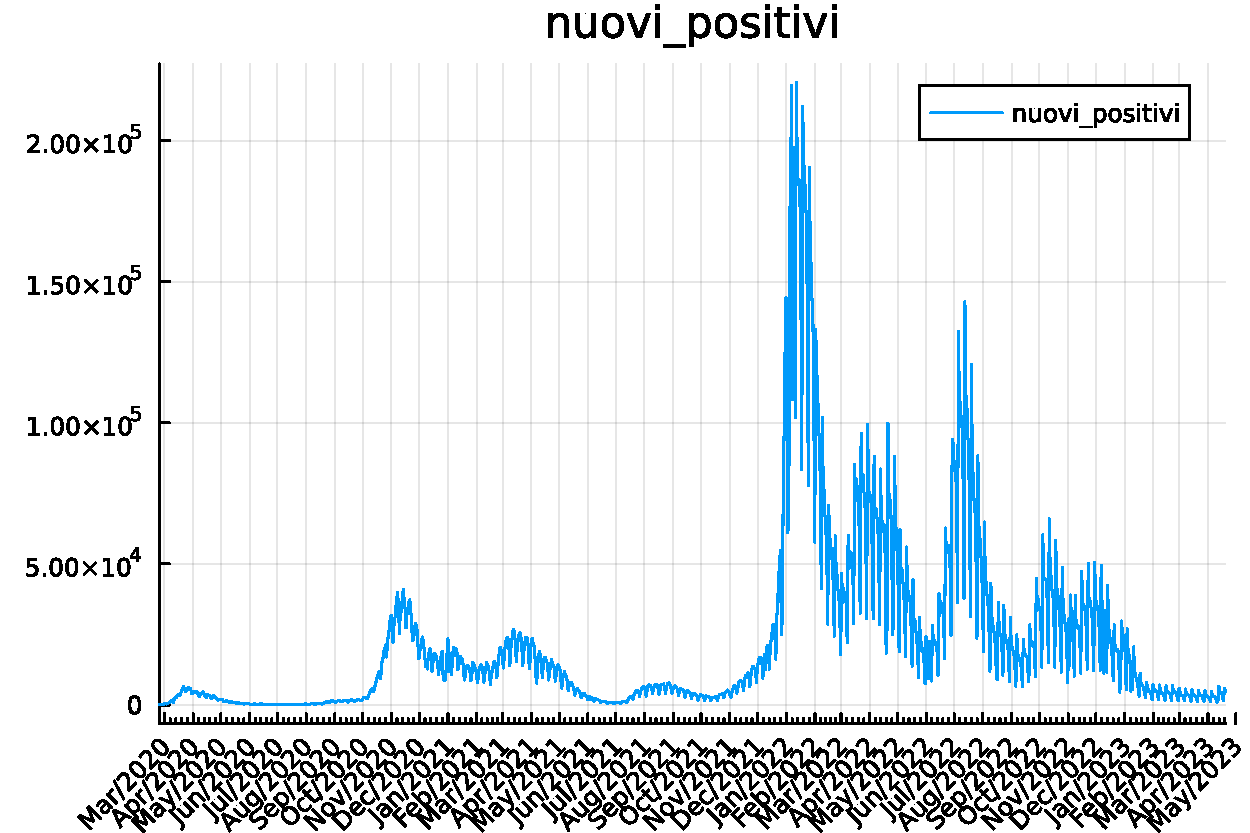
\includegraphics[width=\linewidth]{img/nuovi_positivi_2023-04-21.pdf}
    \caption{Dati sui nuovi positivi dati dal Dipartimento di Protezione Civile Italiana}
    \label{fig:DPC_new_positive}
\end{figure}

Questa tipologia di modello è definita come SEIRS e al suo interno generalmente 
tiene in considerazione un ulteriore stato ovvero quello conosciuto come D, Deceased,
andando quindi a distinguere in maniera chiara gli individui deceduti e quelli invece
guariti. 

\begin{figure}
    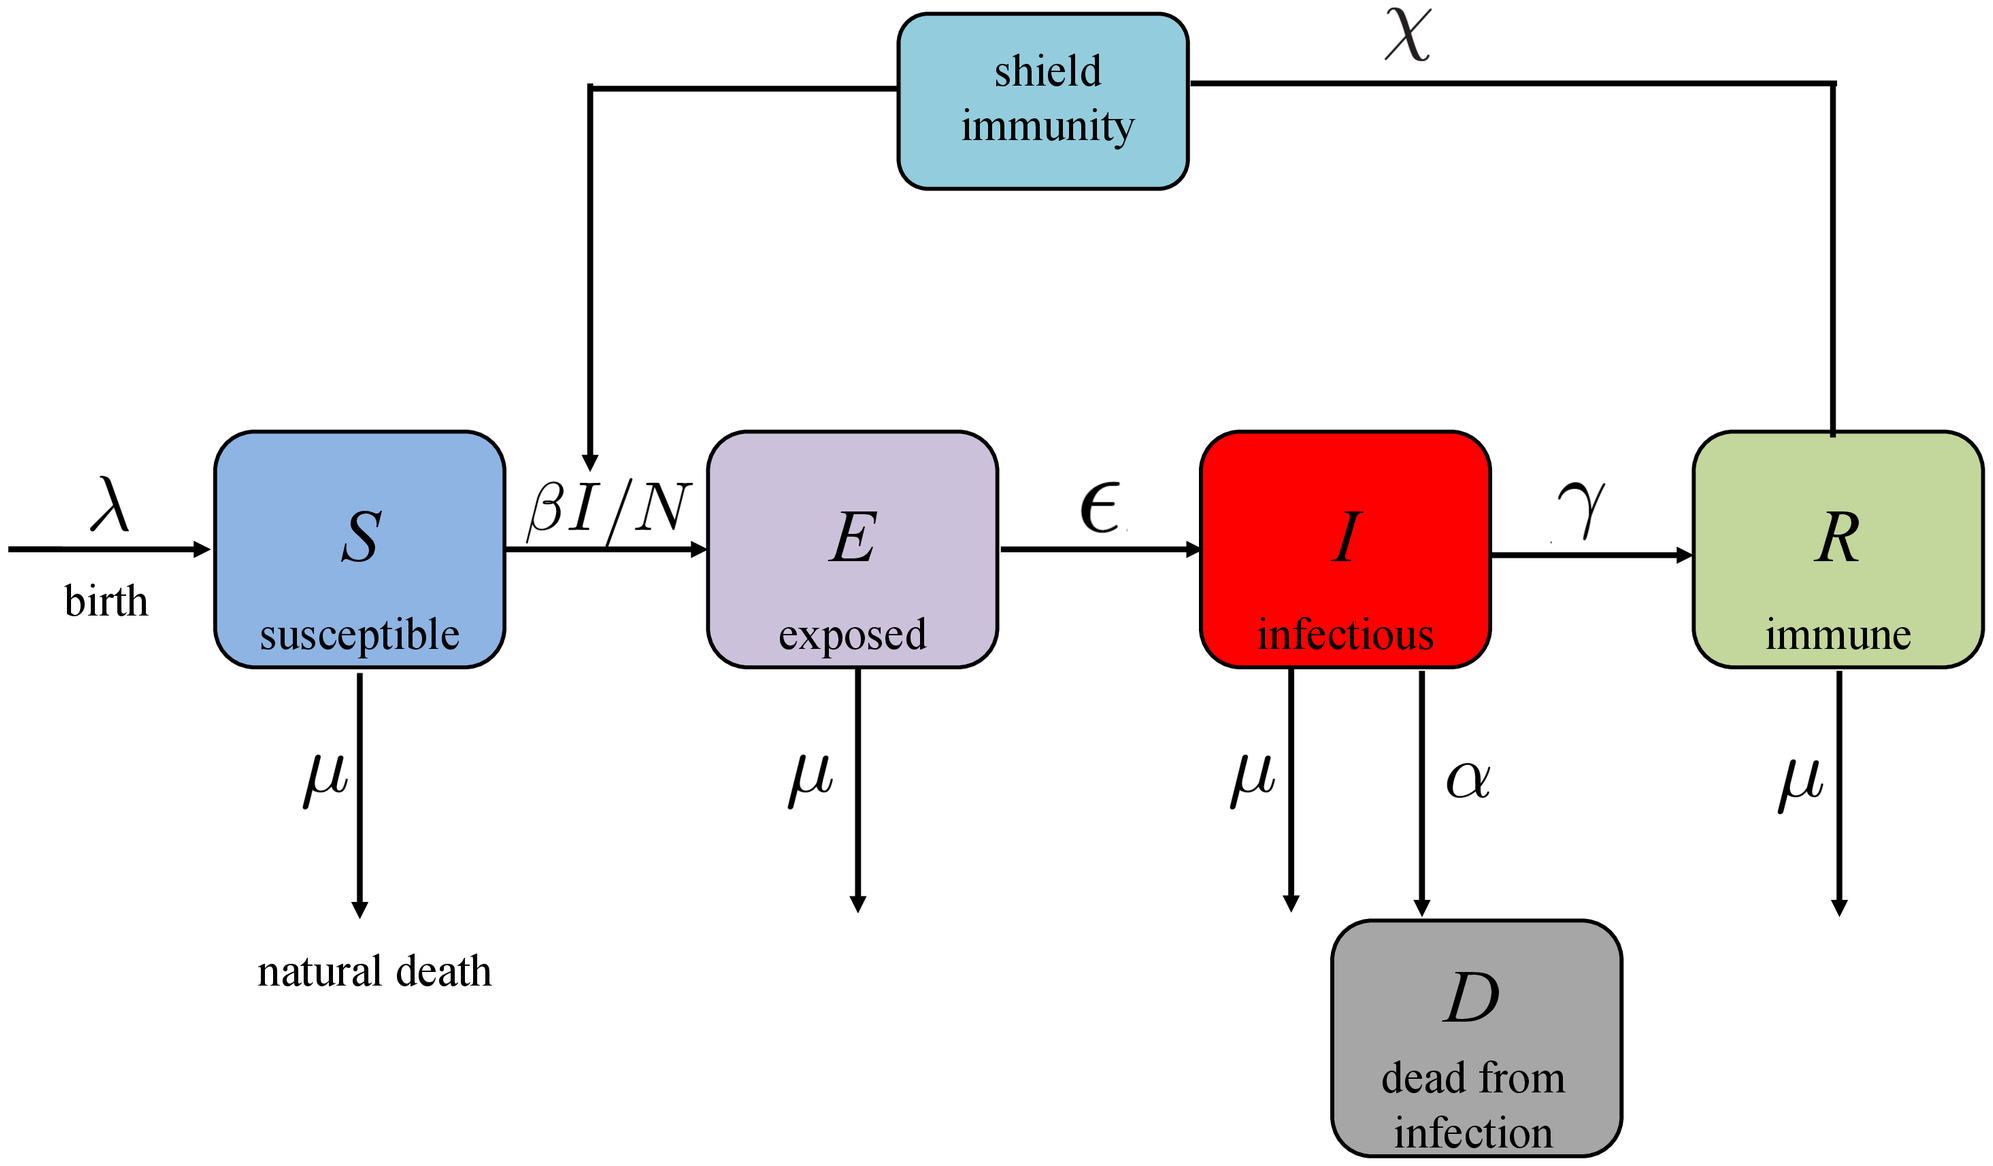
\includegraphics[width=\linewidth]{img/journal.pone.0247660.g002.PNG}
    \caption{Esempio di modello SEIR ciclico con perdita immunità}
    \label{fig:SEIR_ciclic}
\end{figure}

Un ulteriore modifica comune al modello SEIR è quella di aggiungere lo
stato V, Vaccinated, come stato esplicito oppure implicito al modello. Questa 
variazione permette di modellallare l'efficacia di un vaccino una volta introdotto 
all'interno della popolazione, ma più in generale permette di osservare
l'efficacia di una politica di vaccinazione in relazione al numero di vaccinazioni 
effettuatein un determinato periodo di tempo. Questo stato se definito in maniera
implicita è definito come la possibilità di passare dallo stato S allo stato R 
con una data probabilità, mentre in versione esplicita si ha uno stato aggiuntivo
ad-hoc, ad esempio lo stato V.

\begin{figure}
    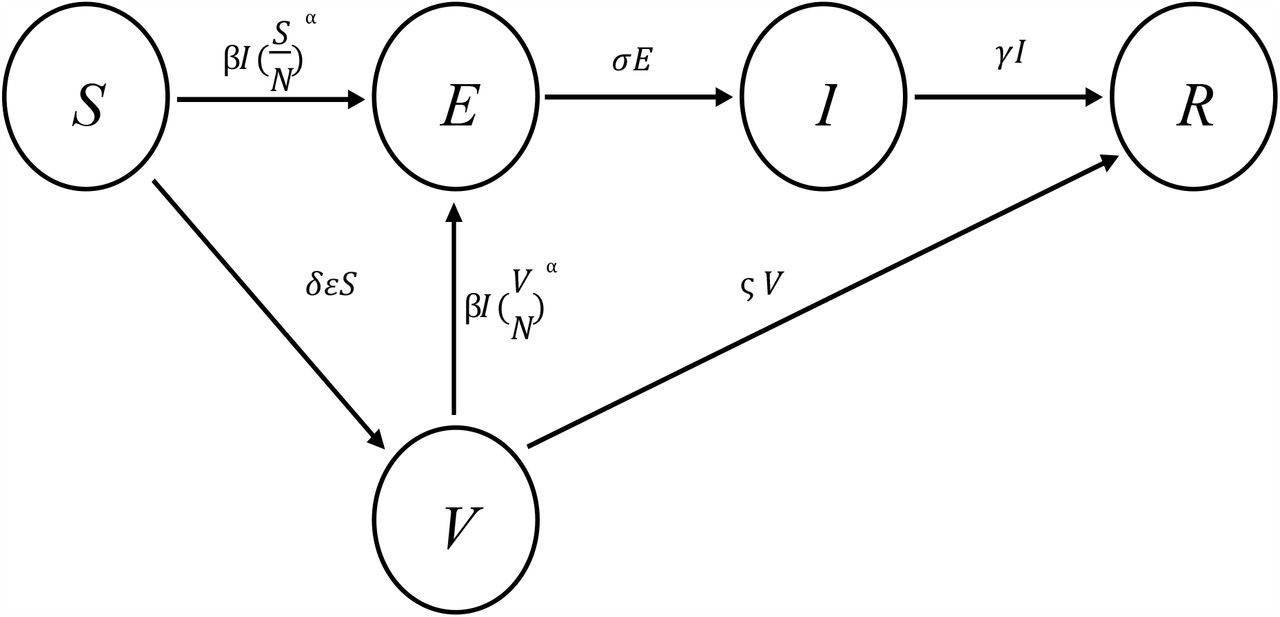
\includegraphics[width=\linewidth]{img/seirv_explicit.jpg}
    \caption{Esempio di modello SEIRV con stato esplicito per la condizione V}
    \label{fig:SEIRV_explicit}
\end{figure}

\begin{figure}
    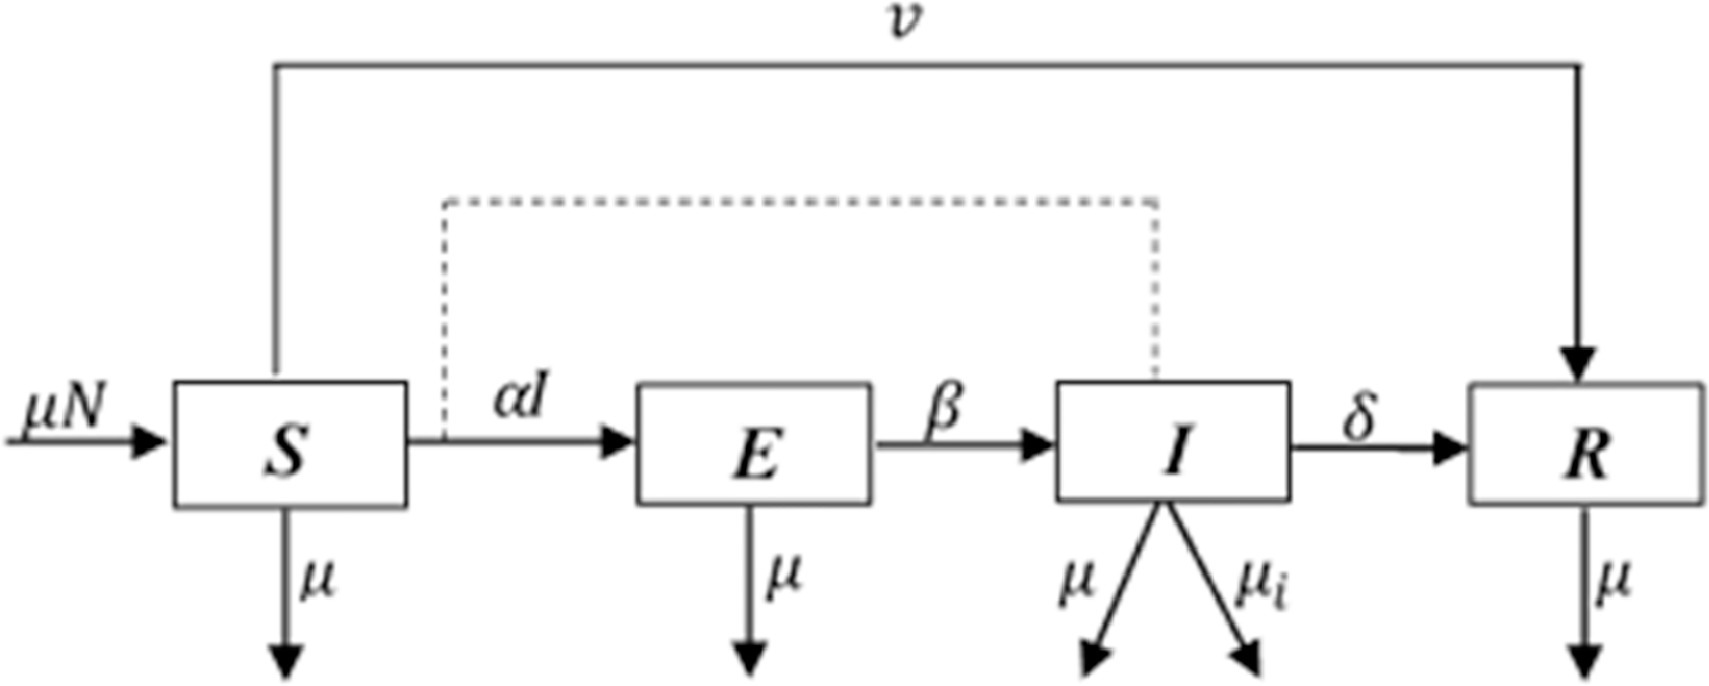
\includegraphics[width=\linewidth]{img/seirv_implicit.jpg}
    \caption{Esempio di modello SEIRV con stato implicito per la condizione V}
    \label{fig:SEIRV_implicito}
\end{figure}

\subsubsection{Modelli Deterministici}
Descrizione dei modelli di tipo deterministico con l'utilizzo delle ODE
Esposizione di alcuni dei modelli utilizzati (principalmente SEIR)

[immagini modelli deterministici]

\subsubsection{Modelli Stocastici}
Descrizione dei modelli di tipo stocastico con l'utilizzo delle SDE
Non ho trovato troppo a riguardo

[immagini modelli stocastici]